\documentclass[conference]{IEEEtran}

\usepackage{cite}
\usepackage{amsmath,amssymb}
\usepackage{graphicx}
\usepackage{booktabs}
\usepackage[T1]{fontenc}

\setlength{\textfloatsep}{4pt}
\setlength{\floatsep}{3pt}
\setlength{\abovecaptionskip}{2pt}
\setlength{\belowcaptionskip}{0pt}
\setlength{\abovedisplayskip}{3pt}
\setlength{\belowdisplayskip}{3pt}
\graphicspath{{../figures/design_window/}}

\begin{document}

\title{Thermal Control Design Windows for Microring WDM Links\\in Co-Packaged AI Optical I/O}

\author{
\IEEEauthorblockN{Yogesh Rethinapandian$^{1}$ and Arun Karthik Sundararajan$^{2}$}
\IEEEauthorblockA{$^{1}$Department of Electrical and Computer Engineering, University of Illinois Chicago, Chicago, IL, USA\\
$^{2}$IEEE Member, USA}
}

\maketitle

\begin{abstract}
Microring WDM links in co-packaged AI optical I/O require active resonance control, but the BER-level detuning window is rarely stated explicitly. We derive control windows for IM/DD PAM4 microring receivers using silicon thermo-optic drift, literature-reported $Q{=}5200$ WDM rings, Lorentzian leakage, true Gray-coded bit counting, and package-informed stress cases. For 100\,GHz WDM at 25\,dB slicer SNR, the residual lock budget is 101--165\,pm, depending on pedestal tracking, to remain below the nominal pre-FEC HD-FEC threshold.
\end{abstract}

\begin{IEEEkeywords}
co-packaged optics, silicon photonics, microring resonator, WDM, thermal drift, resonance locking, PAM4
\end{IEEEkeywords}
\vspace{-5pt}

\section{Introduction}
Co-packaged photonics is moving optical I/O into the thermal neighborhood of compute packages, where packaging and thermal control become system-level constraints rather than device afterthoughts~\cite{mahajan2022,lee2023,matsumoto2022}. Silicon microring resonators (MRRs) are attractive for dense WDM because they are compact and wavelength-selective, but their resonances shift strongly with temperature. Near 1550\,nm, silicon's thermo-optic coefficient gives $d\lambda/dT\approx72$\,pm/$^\circ$C~\cite{komma2012}, comparable to a substantial fraction of practical MRR linewidths.

Prior work has demonstrated MRR tuning and stabilization~\cite{jayatilleka2015}, and recent WDM rings report measured $Q{=}5200$ with 589\,pm/V gate tunability~\cite{hsu2023}. What is still missing for CPO link budgeting is a BER-level answer to: how accurately must the resonance be held after thermal drift and control? This paper contributes a residual detuning window, a Q/spacing/SNR design map, and a package-informed translation from multi-nm drift to sub-linewidth lock accuracy.

\section{Model}
Each MRR drop port is modeled as
\begin{equation}
T_{\rm drop}(\Delta\lambda)=\frac{1}{1+\left(2\Delta\lambda/{\rm FWHM}\right)^2},
\end{equation}
where ${\rm FWHM}=\lambda_0/Q$. Temperature drift is
\begin{equation}
\Delta\lambda_T=\frac{\lambda_0}{n_g}\frac{dn}{dT}\Delta T,
\end{equation}
with $\lambda_0=1550$\,nm, $n_g=4.0$, and $dn/dT=1.86{\times}10^{-4}$\,K$^{-1}$~\cite{komma2012}; thermal expansion is neglected. Eight equal-power WDM channels are placed on 50, 100, or 200\,GHz grids; 100\,GHz is 0.80\,nm near 1550\,nm. For a center drop port, all seven non-selected WDM interferers are Lorentzian-weighted, and we report the worse of positive/negative residual detuning.

We use nonnegative Gray-coded IM/DD PAM4 levels $\{0,1,2,3\}$. SNR is ${\rm Var}(x)/\sigma^2$ at the slicer for an aligned unit-gain channel. The adaptive case tracks the slowly varying mean WDM-leakage pedestal; the fixed-threshold case bounds receivers without pedestal adaptation. BER is computed by enumerating discrete WDM interference and integrating AWGN over PAM4 decision regions. Monte Carlo counts true bit errors. Package stress uses imported CSV data or a disclosed synthetic edge-hotspot scenario motivated by OIF and Ansys CPO workflows~\cite{oif2023,ansys2026}. The design criterion is the nominal pre-FEC HD-FEC BER $=3.8{\times}10^{-3}$.

\begin{table}[!h]
\centering
\caption{Model scope and headline values.}
\label{tab:scope}
\scriptsize
\begin{tabular}{@{}lll@{}}
\toprule
Item & Included/value & Scope/role\\
\midrule
MRR/WDM & Lorentzian, 7 interferers & crosstalk\\
PAM4 BER & Gray bits, AWGN & slicer SNR\\
Not modeled & OMA/RLM, TIA/RIN, EQ & link penalties\\
$Q{=}5200$ FWHM & 298\,pm & linewidth\\
Lock budget & 101--165\,pm & fixed/adaptive\\
\bottomrule
\end{tabular}
\end{table}

\begin{figure}[!t]
\centering
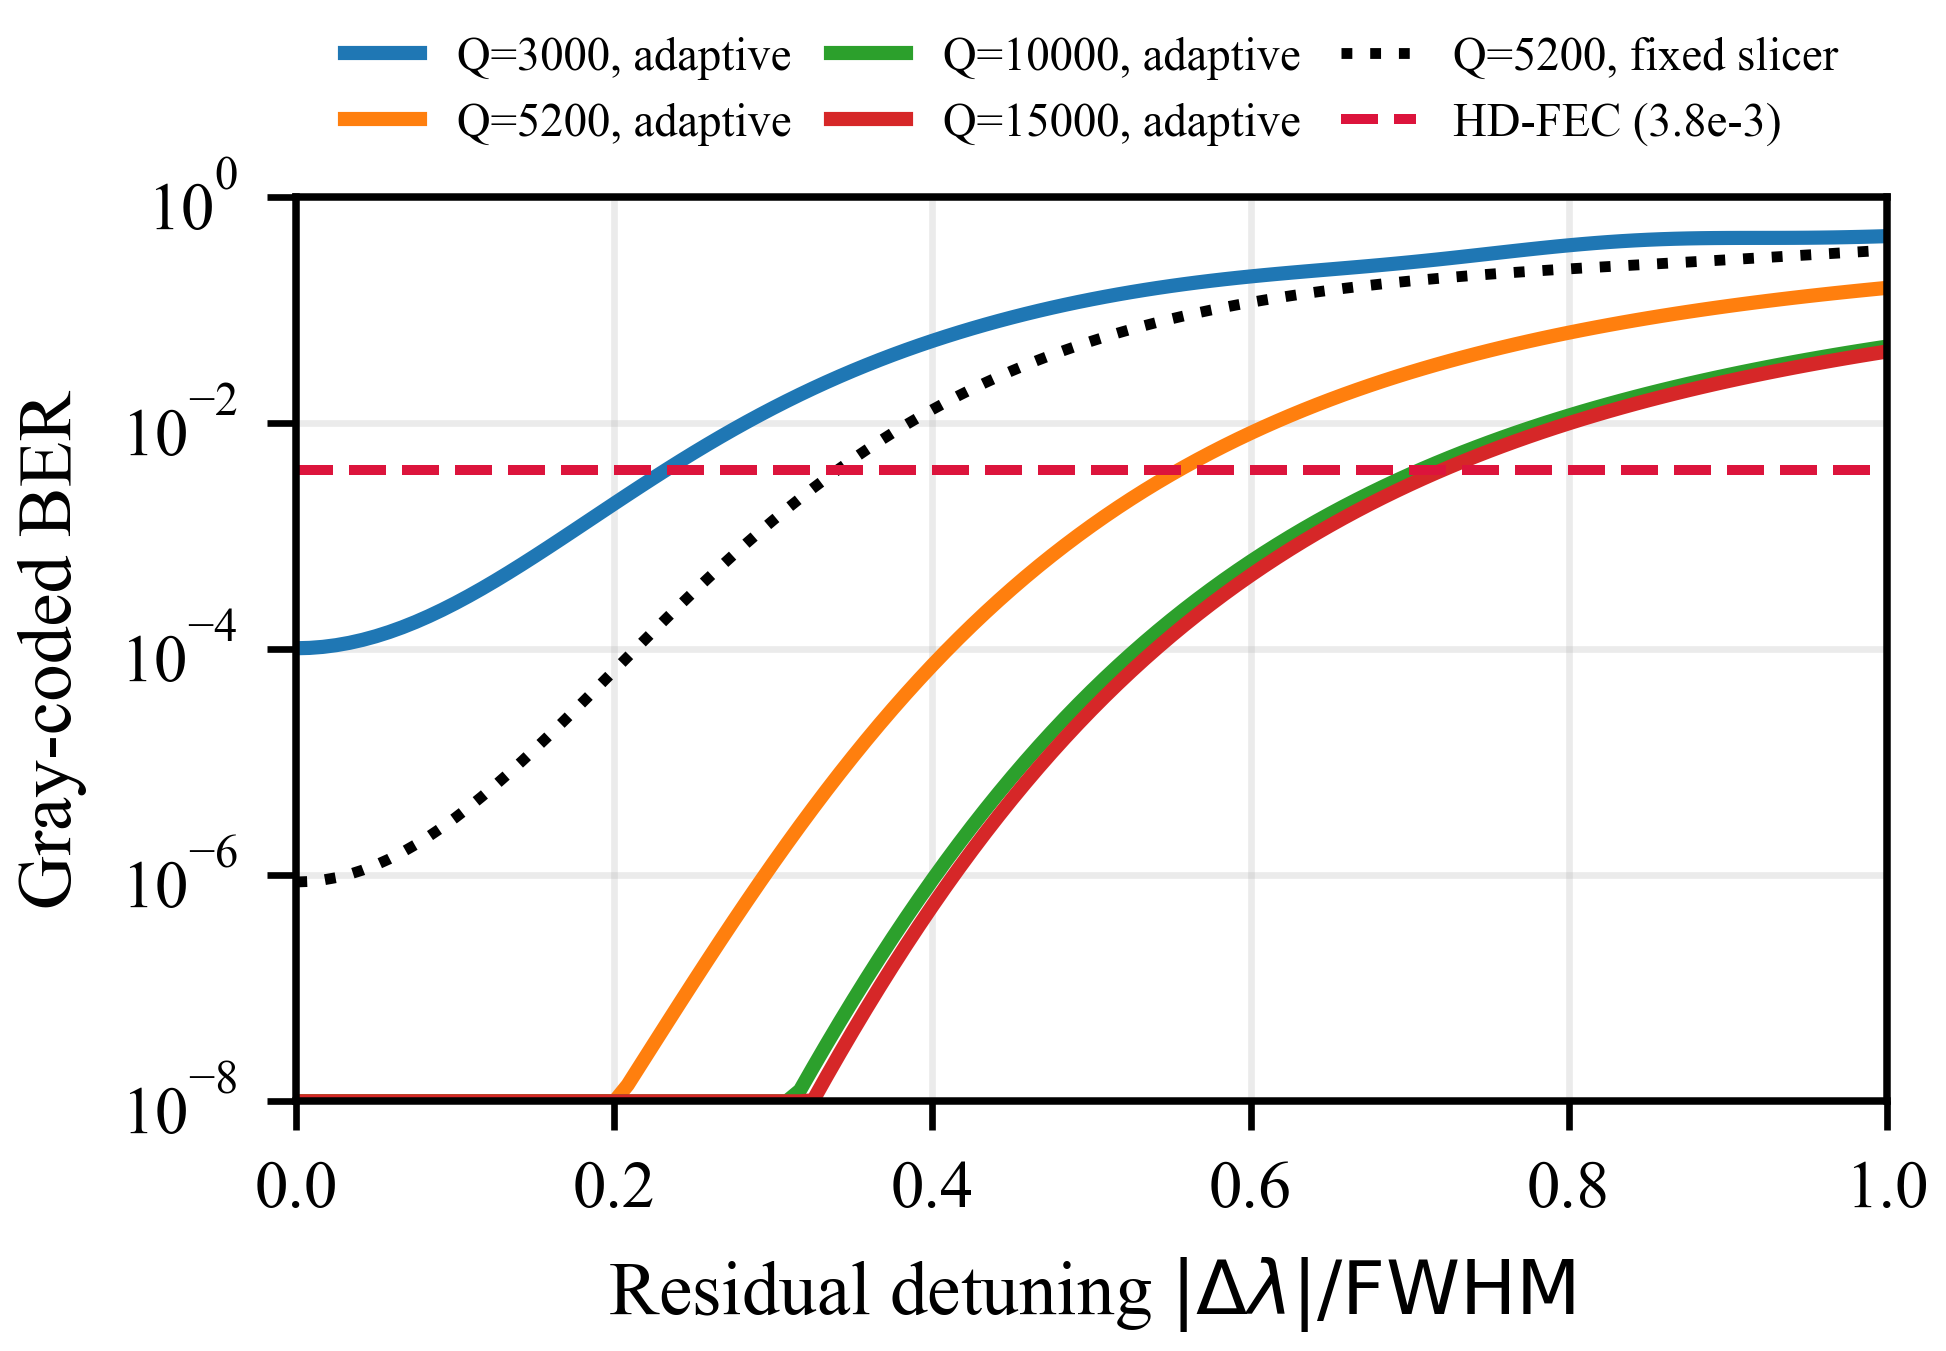
\includegraphics[width=\columnwidth]{paper_fig1_ber_vs_detuning.png}
\caption{Gray-coded BER versus residual resonance detuning for 100\,GHz WDM and 25\,dB electrical slicer SNR under identical Lorentzian-only receiver assumptions. Solid curves use adaptive mean-pedestal tracking; the dotted curve shows the conservative $Q{=}5200$ fixed-threshold receiver.}
\label{fig:ber_detune}
\end{figure}

\section{Results}
Fig.~\ref{fig:ber_detune} shows that the useful control variable is not raw temperature but residual detuning after compensation. At 100\,GHz spacing and 25\,dB slicer SNR, the literature-reported $Q{=}5200$ case remains below HD-FEC to 0.55\,FWHM, equal to 165\,pm or 2.3$^\circ$C equivalent drift. Without mean-pedestal tracking, the same case tightens to 0.34\,FWHM, or 101\,pm. Lower-$Q$ rings are more tolerant in absolute linewidth but suffer more WDM leakage; $Q{=}3000$ allows only 0.23\,FWHM at the same SNR.

\begin{figure}[!t]
\centering
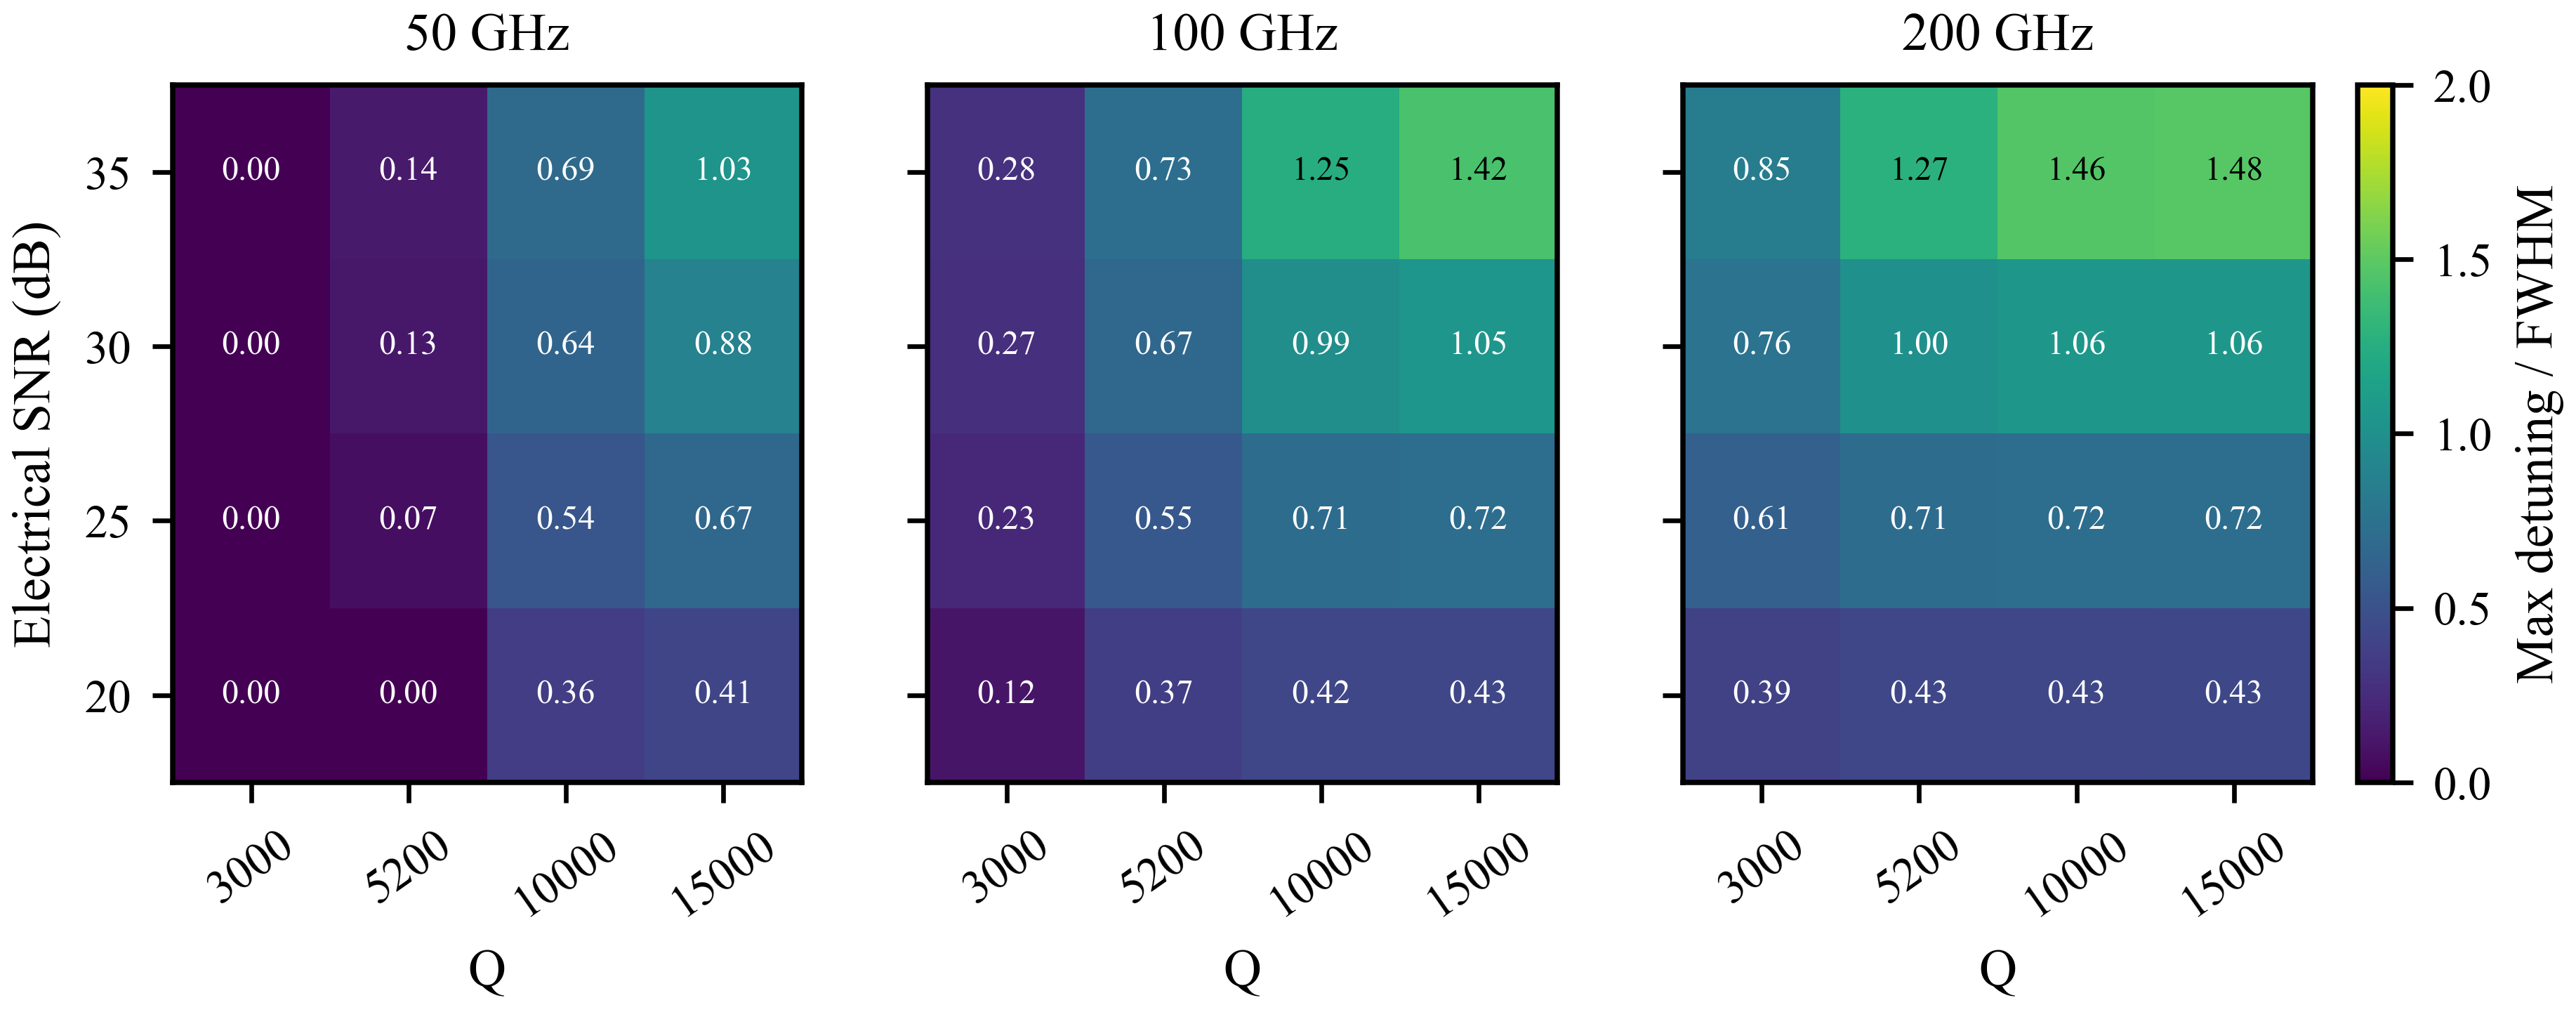
\includegraphics[width=\columnwidth]{paper_fig2_design_window_heatmap.png}
\caption{Residual detuning, in linewidths, that preserves the nominal pre-FEC HD-FEC threshold for 50/100/200\,GHz WDM.}
\label{fig:window}
\end{figure}

The spacing/SNR/Q design window in Fig.~\ref{fig:window} quantifies this tradeoff. At 50\,GHz, low-$Q$ rings have no FEC-compliant residual window under these assumptions because Lorentzian tails dominate even at zero detuning. At 100\,GHz, the $Q{=}5200$ window grows from 0.37 to 0.73\,FWHM over 20--35\,dB SNR. At 200\,GHz, crosstalk is relaxed and the lock budget becomes mainly noise- and linewidth-limited.

\begin{figure}[!t]
\centering
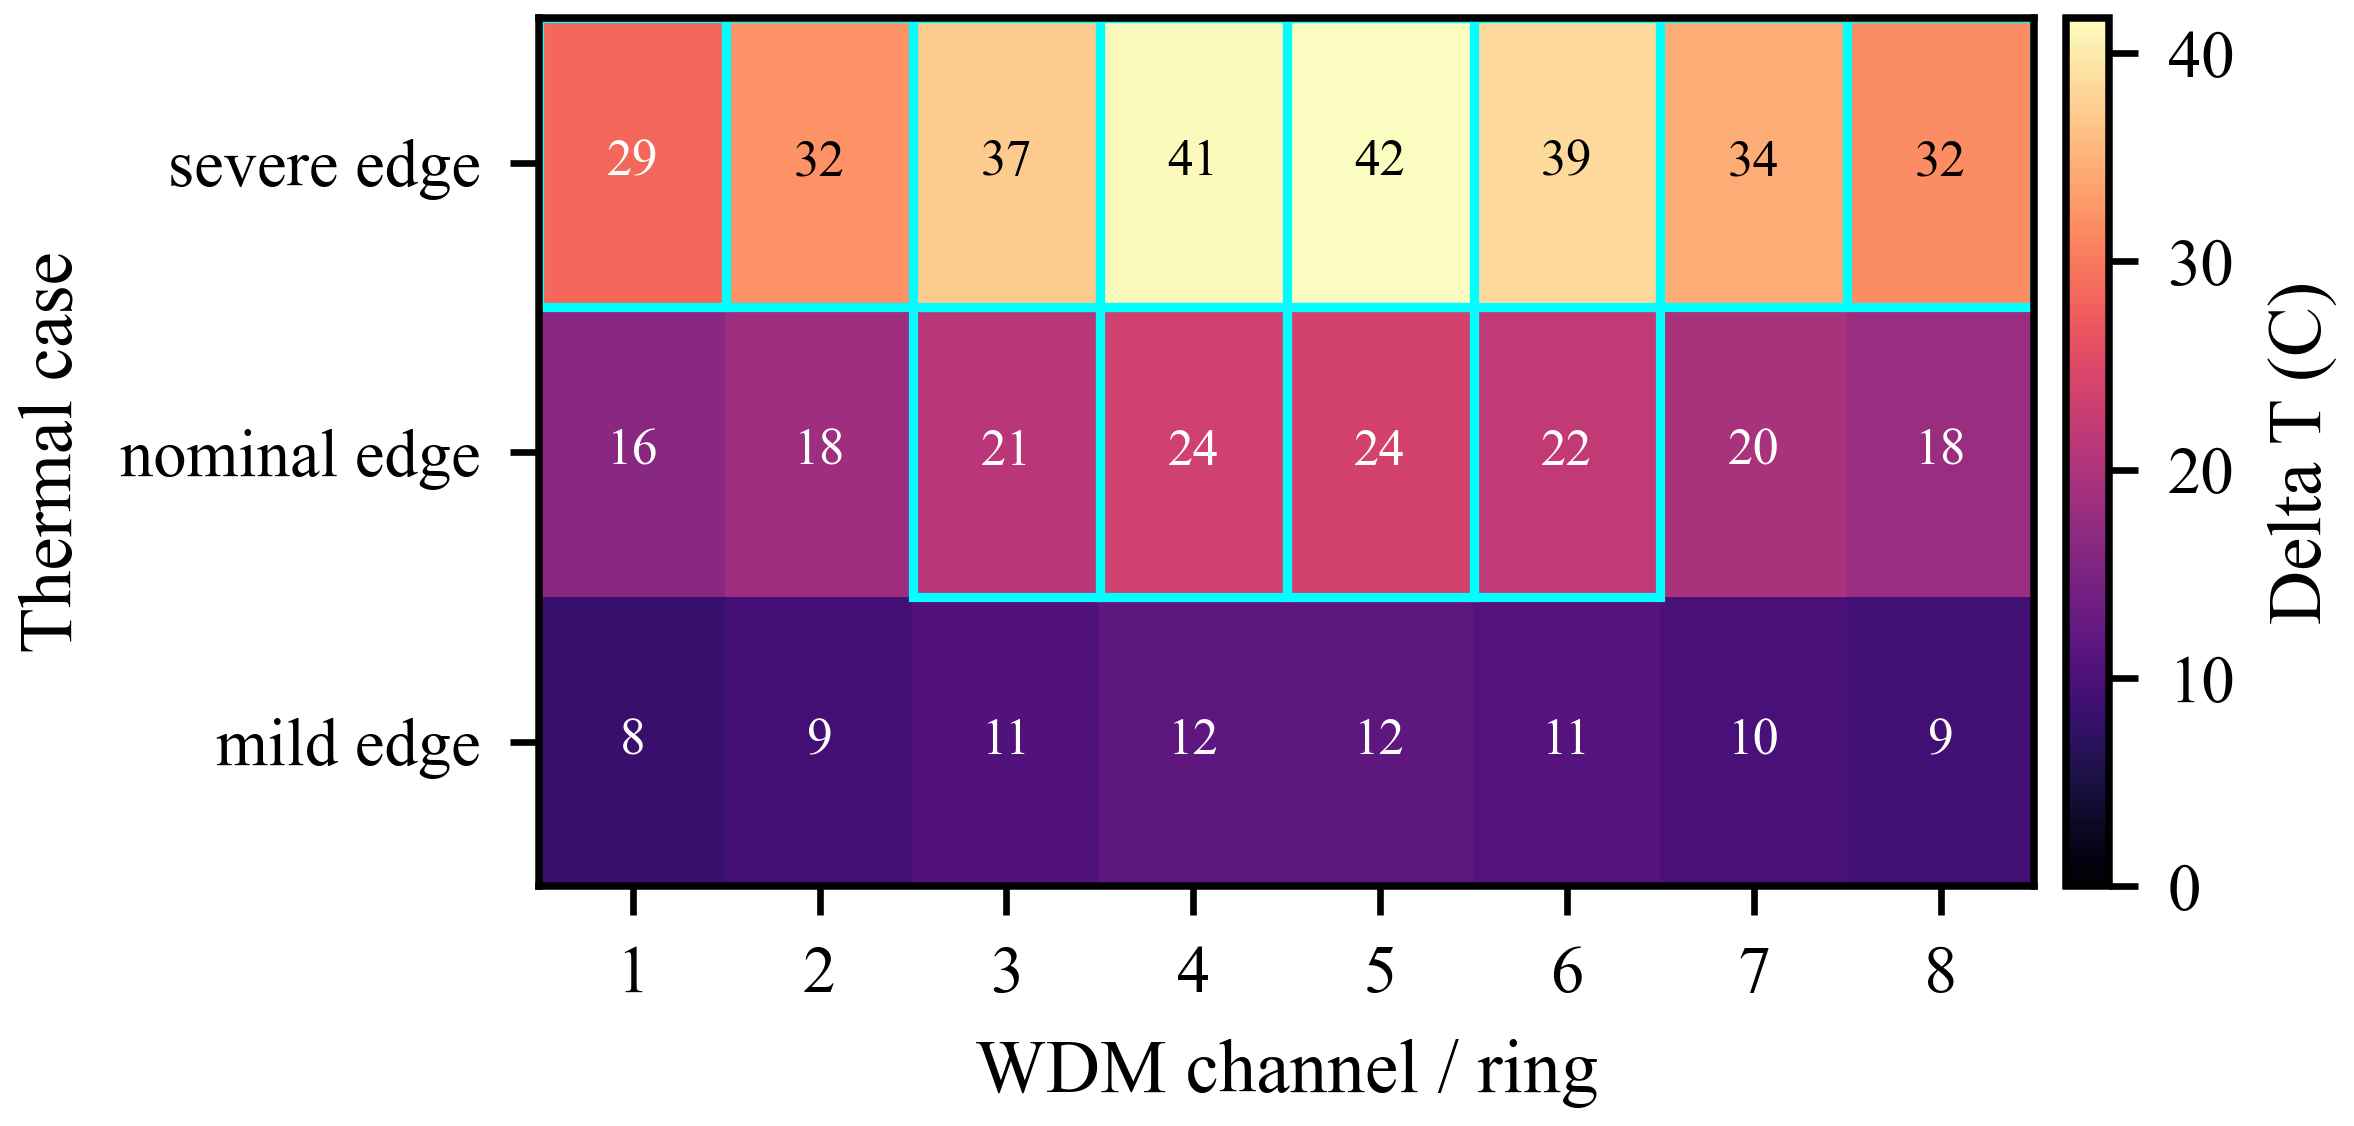
\includegraphics[width=\columnwidth]{paper_fig5_package_thermal_scenarios.png}
\caption{Illustrative package-informed thermal stress cases for an eight-ring optical engine. Cell values are local photonic-layer $\Delta T$ in $^\circ$C; cyan outlines mark $\Delta T\ge20.8^\circ$C, corresponding to $>1.5$\,nm drift at 72\,pm/$^\circ$C.}
\label{fig:package}
\end{figure}

Fig.~\ref{fig:package} illustrates how the BER window maps onto package-scale temperature nonuniformity. OIF estimates that a 3.2\,Tb/s dense optical engine can dissipate 32\,W in a 20$\times$20\,mm$^2$ footprint~\cite{oif2023}, while Ansys demonstrates thermal-map-driven WDM BER simulation~\cite{ansys2026}. Our disclosed synthetic edge-hotspot cases span 8--42$^\circ$C local rise; the 1.5\,nm ITiO range~\cite{hsu2023} is exceeded in the nominal center channels. These illustrative cases show why coarse multi-nm trim and 101--165\,pm closed-loop residual control should be budgeted separately.

\begin{figure}[!t]
\centering
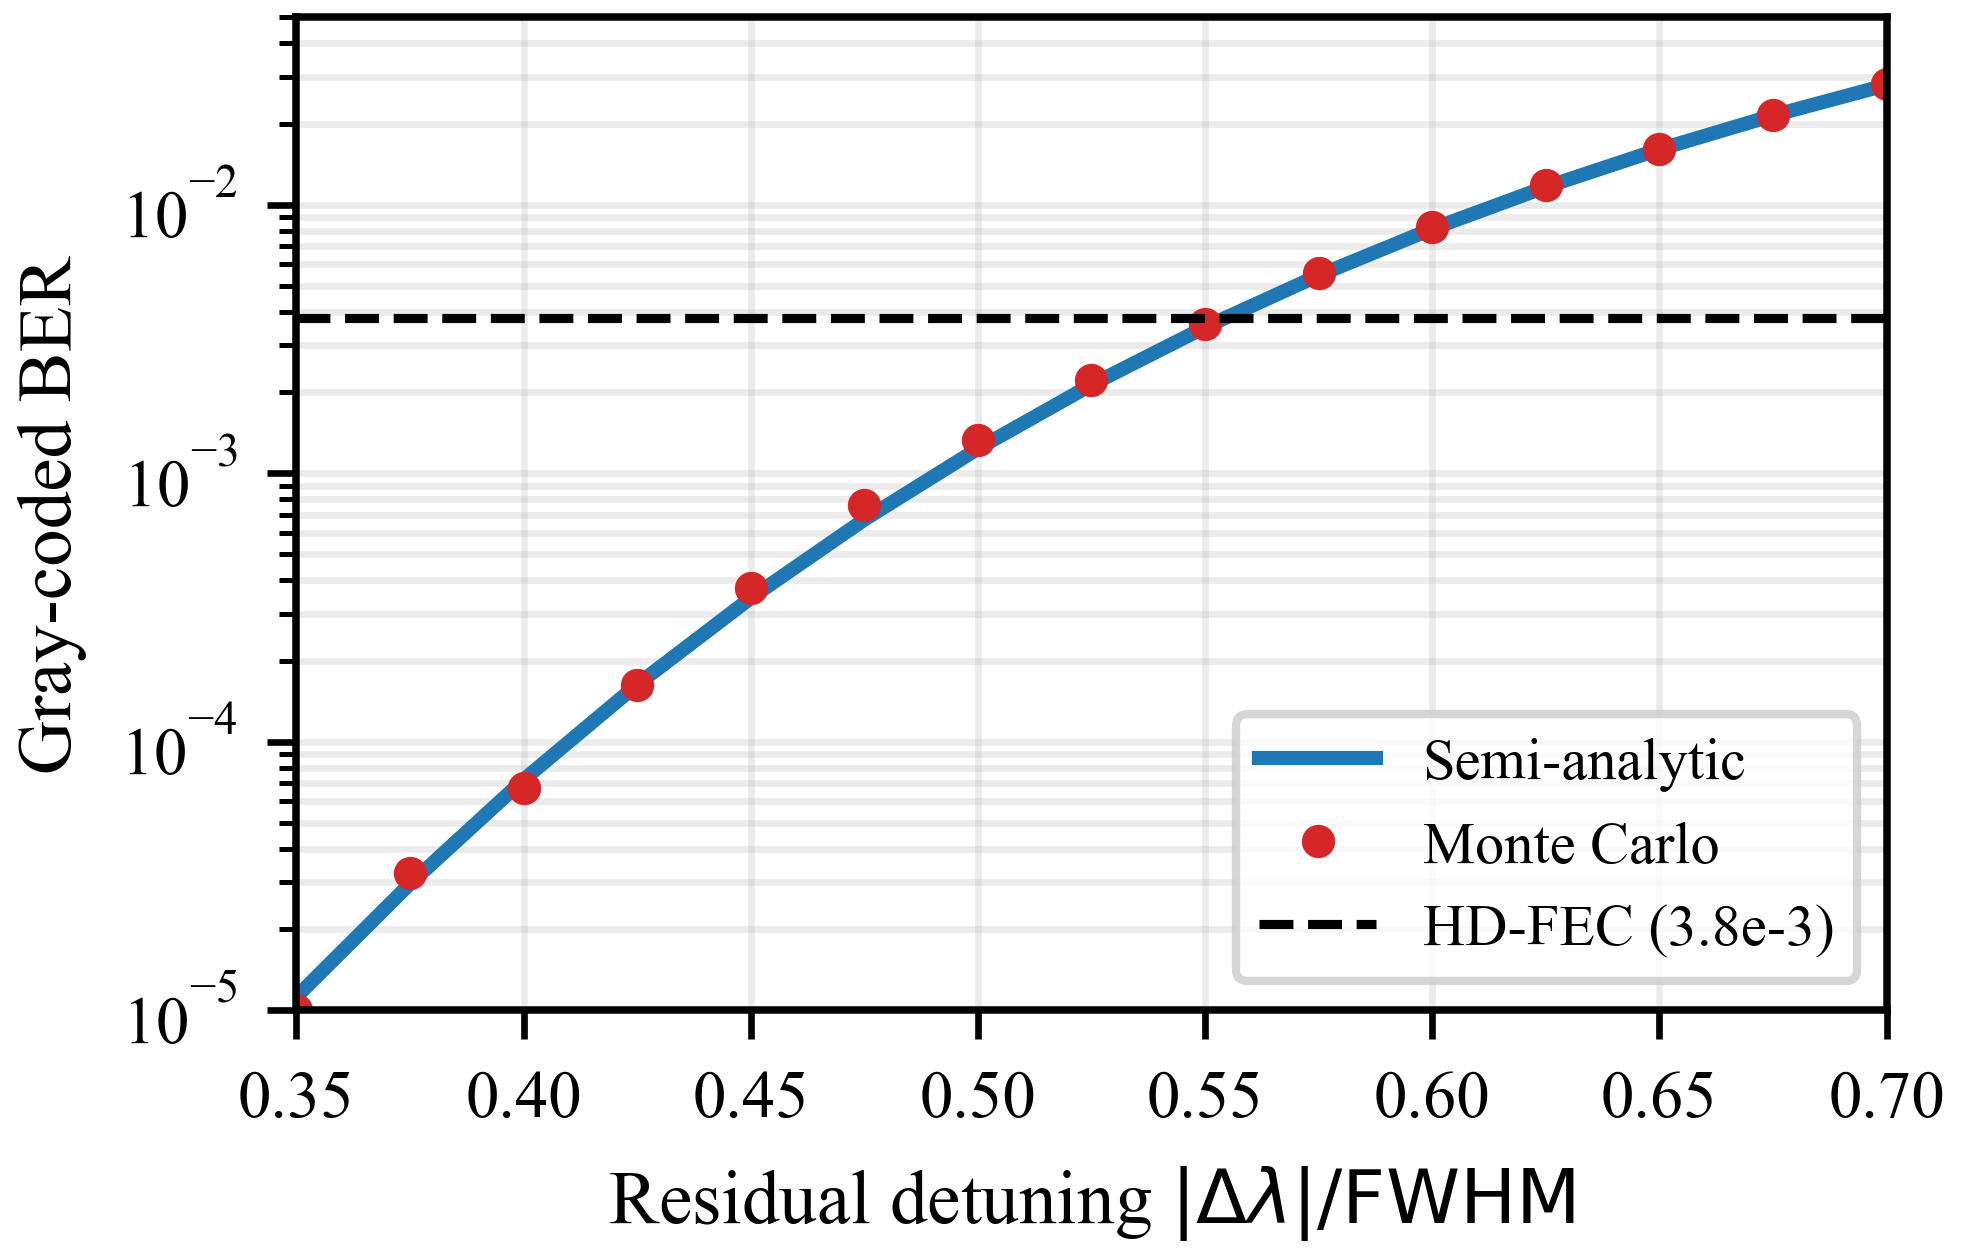
\includegraphics[width=\columnwidth]{paper_fig4_mc_validation.png}
\caption{Near-FEC Monte Carlo cross-check for $Q{=}5200$, 100\,GHz WDM, and 25\,dB slicer SNR. Markers count Gray-coded bit errors over 200,000 PAM4 symbols per point.}
\label{fig:mc}
\end{figure}

Finally, Fig.~\ref{fig:mc} cross-checks the BER implementation against Monte Carlo symbol streams under the same Lorentzian, equal-power, and AWGN assumptions. Agreement near the HD-FEC crossing confirms that the window is not a symbol-error artifact. The model remains first-order: SNR does not separately model OMA, RLM, photodiode responsivity, TIA noise/bandwidth, RIN, equalization, or control-loop dynamics.

\section{Conclusion}
Control-aware BER modeling shows that uncompensated silicon MRR WDM links are not a credible CPO operating mode, but active control can be budgeted quantitatively. For the literature-reported $Q{=}5200$ WDM ring at 100\,GHz spacing and 25\,dB slicer SNR, the residual lock budget is about 100--165\,pm depending on pedestal tracking. Synthetic package-informed stress cases illustrate why practical CPO optical I/O needs coarse tuning range and closed-loop stability.

\begin{thebibliography}{8}
\bibitem{mahajan2022}
R.~Mahajan \textit{et al.}, ``Co-packaged photonics for high performance computing: status, challenges and opportunities,'' \textit{J. Lightw. Technol.}, vol.~40, no.~2, pp.~379--392, 2022.

\bibitem{lee2023}
B.~G. Lee \textit{et al.}, ``Beyond CPO: a motivation and approach for bringing optics onto the silicon interposer,'' \textit{J. Lightw. Technol.}, vol.~41, no.~4, pp.~1152--1162, 2023.

\bibitem{matsumoto2022}
K.~Matsumoto, M.~Farooq, and J.~Knickerbocker, ``Thermal solution for co-packaged optics modules,'' in \textit{Proc. EDAPS}, 2022.

\bibitem{komma2012}
J.~Komma \textit{et al.}, ``Thermo-optic coefficient of silicon at 1550 nm,'' \textit{Appl. Phys. Lett.}, vol.~101, 041905, 2012.

\bibitem{jayatilleka2015}
H.~Jayatilleka \textit{et al.}, ``Wavelength tuning and stabilization of microring-based filters using silicon in-resonator photoconductive heaters,'' \textit{Opt. Express}, vol.~23, no.~19, pp.~25084--25097, 2015.

\bibitem{hsu2023}
W.-C.~Hsu \textit{et al.}, ``On-chip wavelength division multiplexing filters using extremely efficient gate-driven silicon microring resonator array,'' \textit{Sci. Rep.}, vol.~13, Art.~5269, 2023.

\bibitem{oif2023}
OIF, ``Co-packaging framework implementation agreement,'' OIF-Co-Packaging-FD-01.0, 2023.

\bibitem{ansys2026}
Ansys Optics, ``Thermally aware photonic circuit simulation of a WDM transceiver--Icepak integration,'' application example, accessed 2026.

\end{thebibliography}

\end{document}
